\documentclass[a4paper,10pt]{scrartcl}

\usepackage[utf8]{inputenc}
\usepackage[ngerman]{babel}
\usepackage[T1]{fontenc}
\usepackage{amsmath}
\usepackage[section]{placeins}
\usepackage{graphicx}
\usepackage{esvect}




\title{Praktikum B Vorbereitung zu Versuch "fm"}
\author{Leon Machtl und Raphael Lehner}
\date{15.11.2019}

\begin{document}
	\maketitle
	\tableofcontents
	\newpage
	
	\section{Einleitung zum Versuch}
		In diesem Versuch geht es um ferromagnetische Stoffe. Er soll dazu dienen, die grundlegenden Phänomene solcher Stoffe kennenzulernen und zu untersuchen. Von besonderer Wichtigkeit sind dabei die Zusammenhänge zwischen der magnetischen Flussdichte, der magnetisches Feldstärke und der Magnetisiserung. Eine Hall-Sonde dient als Feldmessgerät. Damit wird das Erdmagnetfeld gemessen, sowie die magnetische Feldstärke einer Luftspule ermittelt und anschließend der Einfluss eines Eisenkerns auf das Magnetfeld der Spule untersucht. Außerdem wird das Hystereseverhalten B(H) des Eisenkerns ermittelt.
	
	\subsection{Wichtige Formeln}
		Die magnetischen Eigenschaften von Materie können durch die Magnetisierung \(\vec{M}\) dargestellt werden. Zusammen mit der magnetischen Feldstärke kann man mit ihr die Flussdichte berechnen:
		\begin{align}
		\vec{B}=\mu_{0} (\vec{H} + \vec{M})
		\end{align}
		Dabei ist jedoch zu beachten, dass die Magnetisierung selbst von \(\vec{H}\) abhängt:
		\begin{align}
		\vec{M}=\chi \vec{H} 
		\end{align}
		Dabei bezeichnet \(\chi\) die magnetisches Suszeptibilität. Die magnetische Suszeptibilität ist eine physikalische Größe ohne Einheit, die die Magnetisierbarkeit von Materie in einem externen Magnetfeld angibt. Im einfachsten Fall gibt sie das Verhältnis der Magnetisierung zur Feldstärke an, im Allgemeinen Fall jedoch handelt es sich bei \(\chi\) um einen 3 x 3-Tensor.\\
		Eine weitere Möglichkeit, die magnetische Flussdichte zu berechnen, ist durch diese Formel mit der relativen Permeabilität \(\mu_{r}\) gegeben:
		\begin{align}
		\vec{B}=\mu_{r} \mu_{0} \vec{H} 
		\end{align}
		wobei \(\mu_{r}\) durch
		\begin{align}
		\mu_{r}=1+\chi 
		\end{align} 
		bestimmt werden kann. Da jedoch die Zusammenhänge zwischen \(\vec{B}\) und \(\vec{H}\) sowie \(\vec{M}\) und \(\vec{H}\) im Allgemeinen eben nicht linear sind wie oben, definiert man die Werte besser differentiell:
		\begin{align}
		\mu_{r} \mu_{0}=\mu =\frac{\partial B}{\partial H}
		\end{align}
		\begin{align}
		\chi=\frac{\partial M}{\partial H}
		\end{align}
		\newpage
		
	\subsection{Ferromagnetismus}
		
		Ferromagnetismus bezeichnet eine Art des Magnetismus von Festkörpern und kann dadurch erklärt werden, dass sich die magnetischen Momente der Atome des Stoffes parallel ausrichten, auch dann, wenn sie sich in einem äußerem Magnetfeld befinden und die Temperatur niedriger als die Curie-Temperatur ist. Der Effekt liegt in einer Wechselwirkung zwischen den Atomen, die zur Folge hat, dass die Gesamtenergie des ferromagnetischen Stoffes mit einer solchen Ordnung geringer ist als mit einer ungeordneten Konfiguration, begründet. Ferromagnete behalten ihre magnetische Ordnung also auch entgegen äußerer Einflüsse in gewissem Rahmen bei. Dies bezeichnet man als Remanenz des Ferromagnetismus. Dies lässt sich durch Effekte in zwei Größenordnungen erklären: \\
		mikroskopisch: gleichgerichtete magnetische Ordnung (Elektronenspins)\\
		makroskopisch: Die Anordnung der Weiss'schen Bezirke (siehe nächstes Unterkapitel).
		
	\subsection{Weiss'sche Bezirke}
		
		Häufig entsteht in ferromagnetischen Körpern eine magnetische Struktur aufgrund der Tatsache, dass sich die magnetischen Momente der Atome parallel ausrichten. Diese Struktur bezeichnet man als "Weiss'sche Bezirke". Die "Bezirke" sind Zonen, in denen die magnetischen Momente in die selbe Richtung zeigen und sind meistens nur wenige Kubikmikrometer groß. Wenn ein Körper sehr viel größer ist als die Ausdehnung eines solchen Bezirks, betrachtet man den Körper als homogen magnetisiert. Die effektive Magnetisierung ist dann kleiner als die der einzelnen Bezirke. Heben sich die Magnetisierungen der einzelnen Bezirke gegenseitig auf, nennt man das den entmagnetisierten Zustand des Körpers.
		
	\subsection{Hysteresekurve}
	
		In einer Hysteresekurve wird die magnetische Flussdichte \(B\) gegen die magnetische Feldstärke \(H\) aufgetragen. Dabei wird der Strom zeitlich verändert:
		\begin{align}
		I(t)=I_{0}t
		\end{align}
		Dabei ändert sich auch die magnetische Feldstärke:
		\begin{align}
		H(t)=H_{0}t
		\end{align}
		Aufgrund von magnetischen Anisotropien und komplexer Dynamik der Weiss'schen Bezirke verläuft die Hysteresekurve nicht gleichmäßig, sondern wie in der Abbildung (siehe Aufgabe 7) .B verhält sich wie folgt:
		\begin{align}
		B=\mu_{0}H+M_{max}
		\end{align}
		Wenn H hohe Werte annimmt, verändert sich B also nur noch langsam, da sich alle magnetischen Dipole ausgerichtet haben und somit \(M_{max}\) konstant ist. Tritt dieser Fall ein, nennt man das magnetische Sättigung. Wird H wieder verringert, folgt B nicht der bisherigen Kurve.
		\newpage
		
	\subsection{Messung von \(\vec{B}\) und \(\vec{H}\) im Quer- und Längsspalt}
	
		Eine direkte Messung der beiden Felder ist in festen Stoffen mit einer makroskopischen Messsonde offensichtlich nicht wirklich möglich, daher misst man mit kalibrierten Hall-Sonden in Hohlräumen der ferromagnetischen Proben. Dabei muss man darauf achten, dass der Feldverlauf in der Probe durch die Hohlräume möglichst wenig gestört wird. Mit den im Folgenden aufgeführten Formeln, die aus den Maxwellgleichungen folgen, kann man mit den Messonden in den Hohlräumen auf die magnetische Flussdichte \(\vec{B}\) und die magnetische Feldstärke \(\vec{H}\) im Festkörper schließen.\\
		\\
		Querspalt (Spalt liegt senkrecht zu H):\\
		Da \(\vec{B}\) quellenfrei ist, folgt unter der Annahme, dass Streufelder und entmagnetisierende Felder vernachlässigbar sind und eine homogene Magnetisierung vorliegt nach kurzer Rechnung und Anwendung des Gaußschen Satzes:
		\begin{align}
		\vec{B_{E}}=\vec{B_{L}}
		\end{align}
		wobei die linke Seite die magnetische Flussdichte im ferromagnetischen Stoff (z.B. Eisen) und die rechte Seite die magnetische Flussdichte im Luftspalt darstellt. Somit erhält man bei der Messung von \(B_{L}\) mit einer transversalen Hall-Sonde direkt den Wert von \(B_{E}\), den man sucht.\\
		\\
		Längsspalt (Spalt liegt parallel zu H):\\
		Da die Wirbel der magnetischen Feldstärke \(\vec{H}\) makroskopischen Strömen mit einer Dichte \(\vec{j}\) entsprechen, kann man mit den selben Annahmen wie beim Querspalt und mit dem Wissen, dass hier die Stromdichte im Eisen und in der Luft 0 ist über eine rechteckige Fläche die teilweise durch das Eisen und teilweise durch die Luft verläuft, integrieren und erhält mit Hilfe des Stokesschen Satzes die Beziehung:
		\begin{align}
		\vec{H_{E}}=\vec{H_{L}}
		\end{align}
		Was analog zu oben den magnetischen Feldstärken im Eisen und in der Luft entspricht. Somit kann man mit einer longitudinalen Hall-Sonde die magnetische Flussdichte im Eisen bestimmen um über folgende Beziehung, die aus Gleichung (3) folgt, die magnetische Feldstärke im Eisen zu berechnen:
		\begin{align}
		H_{E}=H_{L}=\frac{1}{\mu_{0}}B_{L}
		\end{align}
		
	\subsection{Der magnetische Kreis}
	
		Ein magnetischer Kreis besteht aus k Elementen mit der länge \(l_{k}\) mit den Querschnittsflächen \(f_{k}\). Dabei gilt, dass es näherungsweise keinen Streufluss gibt, es also gilt:
		\begin{align}
		\phi_{k}=B_{k}f_{k}=const.
		\end{align}
		\(\phi\) wird auch magnetischer Strom genannt.
		Es besteht somit eine Ähnlichkeit zu einem Stromkreis, bei dem überall der gleiche Strom fließt. Die magnetische Spannung ergibt sich durch:
		\begin{align}
		nI=\sum_{k}^{}H_{k}l_{k}
		\end{align}
		wobei \(n\) die Windungszahl der Spule ist und \(I\) der Spulenstrom. Folgender Ausdruck wird als magnetischer Widerstand bezeichnet:
		\begin{align}
		R_{mag}:=\sum_{k}^{}\frac{l_{k}}{\mu_{0}\mu_{k}f_{k}}
		\end{align}
		Somit folgt das Ohmsche Gesetz des Magnetischen Kreises:
		\begin{align}
		nI=\phi R_{mag}
		\end{align}
		Der im Experiment verwendete Eisenkern lässt sich  als Torus beschreiben. Somit gilt nach Gleichung (14)
		\begin{align}
		H(r)=\frac{nI}{2\pi r}
		\end{align}
		Wird der Eisenkern durch einen Querspalt unterbrochen, so erhält man unter Vernachlässigung von Streufeldern diese Zusammenhänge:
		\begin{align}
		\vec{B_{E}}=\mu_{0}(\vec{H_{E}}+\vec{M})
		\end{align}
		\begin{align}
		\vec{B_{L}}=\mu_{0}\vec{H_{L}}
		\end{align}
		Aus Gleichung (10) folgt dann
		\begin{align}
		\vec{H_{L}}=\vec{H_{E}}+\vec{M}
		\end{align}
		Somit gilt für die hier vorliegende Situation:
		\begin{align}
		nI=H_{L}l_{L}+H_{E}l_{E}
		\end{align}
		Aus obigen Gleichungen folgt:
		\begin{align}
		B_{E}=B_{L}=\mu_{0}(\frac{nI}{l}+M\frac{l_{E}}{l})
		\end{align}
		Für kleine \(l_{L}\) wird also die magnetische Flussdichte durch den Eisenkern um \(\mu_{0}\) mal die Magnetisierung verstärkt. Es folgt außerdem:
		\begin{align}
		H_{E}=(\frac{nI}{l}-M\frac{l_{L}}{l})
		\end{align}
		Also wird das magnetisierende Feld durch den Luftspalt verringert.
		
		\newpage
		
	\subsection{Induktionsgesetz}
	
		Aus der Formel für den magnetischen Fluss durch eine Fläche A senkrecht zur magnetischen Flussdichte B ergibt sich die Formel für den Fluss in einem ringförmigen Eisenkern in einer stromdurchflossenen Spule mit N Windungen:
		\begin{align}
		\phi=AB=A\mu_{r}\mu_{0}H=A\mu_{r}\mu_{0}\frac{NI}{l}
		\end{align}
		wobei A der Querschnitt des Eisenkerns. Durch eine Änderung des Flusses wird eine Spannung induziert:
		\begin{align}
		V_{ind}=-N_{m}\frac{\partial \phi}{\partial t}=-N_{m}N\frac{A}{l}\mu_{0}\frac{\partial \mu_{r}I}{\partial t}
		\end{align}
		wobei \(N_{m}\) die Windungszahl einer zusätzlichen Spule bezeichnet, die genutzt wird um die induzierte Spannung abzugreifen (Induktionsspule). Durch Integration der Induktionsspannung über die Zeit erhält man:
		\begin{align}
		\int_{0}^{t}V_{ind}dt'=-N_{m}A[B(t)-B(0)]=-N_{m}[\phi(t)-\phi(0)]
		\end{align}
		Es ist also möglich, durch die Integration der Induktionsspannung die magnetischen Flüsse zu messen. Wenn A bekannt ist, erhält man auch die magnetische Flussdichte B.
	
	

\section{Aufgaben zur Vorbereitung}

\subsection{Aufgabe 1}
Einheitenbetrachtung wichtiger Größen des Versuchs:
\begin{itemize}
	\item Magnetische Flussdichte $[\vec{B}]=1~\frac{Vs}{m^2}=1~T$
	\item Magentische Feldstärke $[\vec{H}]=1~\frac{A}{m}$
	\item Magentisiertung $[\vec{M}]=1~\frac{A}{m}$
	\item Magnetischer Fluss $[\Phi]=1~Tm^2=1~Vs=1~Wb$
	\item Magnetische Permeabilität $[\mu_r]=1$
	\item Magnetische Feldkonstante $[\mu_0]=1~\frac{Vs}{Am}$ 
	\item Stromdichte $[\vec{j}]=1~\frac{A}{m^2}$
\end{itemize} 

\subsection{Aufgabe 2}
Wie lautet der Zusammenhang zwischen $\mu$ und $\chi$?\\
Aus Gleichung (3) folgt $\mu$ = $\mu_r$$\mu_0$. \\
Weiterhin gilt mit Gleichung (4) $\mu_r$ = 1 + $\chi$. \\
Eingesetzt folgt somit $\mu$ = (1 + $\chi$) $\mu_0$

\subsection{Aufgabe 3}
Beschreibung der Unterschiede zwischen Diamagnetismus, Paramagnetismus und Ferromagnetismus: \\
Diamagnetismus: Diamagnetische Materialien induzieren beim Anlegen eines äußeren Magnetfelds ein Magnetfeld, das dem äußeren Magnetfeld entgegenwirkt. Sie bewegen sich somit aus einem Magnetfeld heraus. Bei besonders starken Magnetfeldern und leichten diamagnetischen Materialien kann es vorkommen, dass die Abstoßung der diamagnetischen Kreisströme die Gewichtskraft kompensiert und sich die Objekte im Magnetfeld bewegen. \\
Paramagnetismus: Paramagnetische Materialien induzieren beim Anlegen eines äußeren Magnetfelds ein Magnetfeld, das in die gleiche Richtung wie das äußere Magnetfeld wirkt. Um diese Eigenschaft zu zeigen, muss ein Stoff ungepaarte Elektronen, freie Atome oder Ionen mit nur teilweise gefüllten Schalen besitzen, damit sich die normalerweise 2 Spins (siehe Pauli) nicht gegenseitig aufheben, sondern das Feld im Inneren verstärken. \\
Ferromagnetismus: Ferromagnetische Materialien enthalten innere magnetische Momente, die auch ohne ein äußeres Magnetfeld parallel ausgerichtet sein können.
\subsection{Aufgabe 4}
$\mu_r$ für magnetische Materialien: \\ \\
\begin{tabular}{|c|c|c|} \hline
	 & $\mu_r$ & X \\ \hline
	diamagnetisch & 0<...<1 & -1<...<0 \\ \hline
	paramagnetisch & >1 & >0 \\ \hline
	ferromagnetisch & >>1 & >>1 \\ \hline
	Vakuum & 1 & 0 \\ \hline
\end{tabular} \\ \\ \\
Supraleiter (ideal diamagnetisch): $\mu_r$ = 0 \\
Vakuum (neutral): $\mu_r$ = 1 \\
Luft (paramagnetisch):  $\mu_r$ = 1 + 4 * $10^{-7}$ \\
Eisen (ferromagnetisch):  $\mu_r$ = 300 - 10000 \\
\subsection{Aufgabe 5}
Parallelität der Vektoren $\vec{B}$ und $\vec{H}$: \\
Für magnetisch isotrope Materialien sind die Vektoren stets parallel. \\
Bei anisotropen Materialien werden die Vektoren laut Skript mit einem Tensor verknüpft.
\subsection{Aufgabe 6}
Größe der "differentiellen Permeabilität" $\frac{\partial B}{\partial H}$, wenn die Sättigungsmagnetisierung erreicht ist: \\
Für die Sättigungsmagnetisierung gilt: \\
\begin{align*}
\frac{\partial \vec{B}}{\partial \vec{H}} = \frac{\partial}{\partial \vec{H}} \mu_0 (\vec{H} + \vec{M}) = \mu_0 \frac{\partial \vec{H}}{\partial \vec{H}}+ \mu_{0} \frac{\partial \vec{M}}{\partial \vec{H}} = \mu_0 + 0 = \mu_0 
\end{align*}
\subsection{Aufgabe 7}
Qualitative Skizze von B(H) und M(H): 
\begin{figure}[h]
\centering
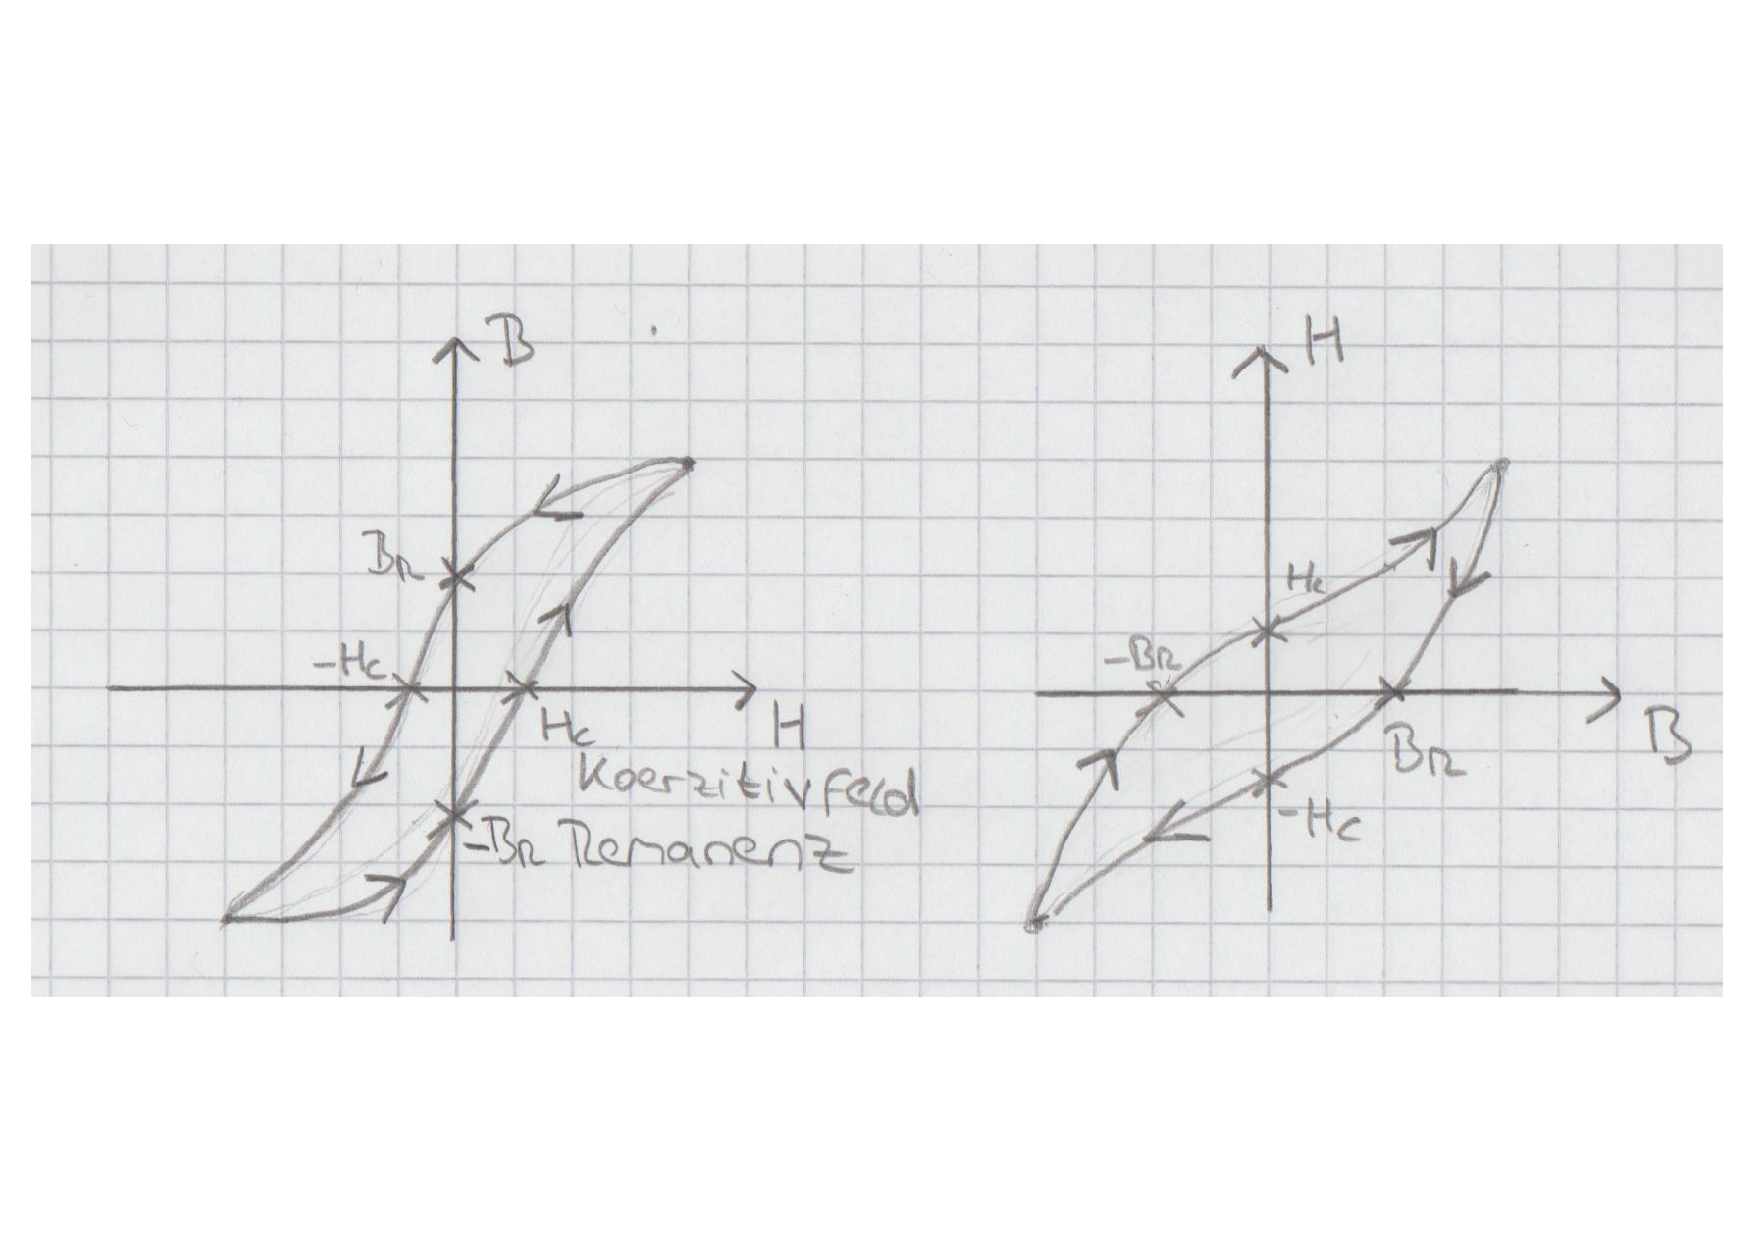
\includegraphics[width=0.9\textwidth]{./Bilder/fmhysterese}
\caption{Hysteresekurve}
\end{figure}
\FloatBarrier
Beide Graphen sind Hysteresekurven, allerdings ist die Richtung der Hysterese entgegengesetzt (siehe Abb. 1).
\subsection{Aufgabe 8}
Wie kann man einen ferromagnetischen Körper in einen "entmagnetisierten Zustand" bringen? \\
Dies wird erreicht, indem man den Körper höher als seine Curie-Temperatur $T_C$ erhitzt. Dabei sortieren sich die magnetischen Momente des Materials neu und gehen in einen energetisch günstigeren, entmagnetisierten Zustand. Eine weitere Möglichkeit stellen das Entmagnetisieren durch starke Erschütterungen und das Anlegen einer Wechselspannung, die langsam auf Null reduziert wird, dar.
\subsection{Aufgabe 9}
Querspalt und Längsspalt bei Magneten \\
Ein Querspalt im Magneten ist senkrecht zu den Feldlinien von $\vec{B}$ und $\vec{H}$ orientiert. Zur Messung der Feldstärke im Inneren des Querspalts und damit auch im Inneren des Materials wird eine transversale Hallsonde verwendet.
Ein Längsspalt dagegen verläuft parallel zu den Feldlinien des Magnetfelds. Sein Magnetfeld wird mit einer longitudinalen Hallsonde gemessen.
\subsection{Aufgabe 10}
Warum müssen die Spalte zur Messung von $\vec{B}$ und $\vec{H}$ in ferromagnetischem Material möglichst eng sein? \\
Bei breiteren Spalten würde es zu stärkeren Streufeldern kommen, die die Messung von $\vec{B}$ und $\vec{H}$ verfälschen würden.
\subsection{Aufgabe 11}
Ist $\vec{B}$ in einem nicht-durchgehenden Querspalt genauso groß wie in einem durchgehenden? \\
In einem durchgehenden Querspalt fällt das $\vec{B}$-Feld, also die magnetische Flussdichte, stärker ab.
\subsection{Aufgabe 12}
Wirkungsweise einer Hallsonde: \\
Eine Hallsonde ist ein Leiter, auf dessen Ladungsträger im Magnetfeld die Lorentzkraft wirkt, sodass die Ladungsträger abgelenkt werden. Diese Ablenkung erzeugt die sogenannte Hallspannung $U_H$, die mit der Hallsonde gemessen wird und aus der die magnetische Flussdichte berechnet werden kann. \\
Geometriebedingte Nullfeldsignale kann man durch eine angelegte Gegenspannung vermeiden.
\subsection{Aufgabe 13}
Das Magnetfeld einer langen Zylinderspule fällt zu den Spulenden hin ab. \\
Wir sollen die Größe des Feldes an den Spulenenden im Vergleich zur Feldstärke im Mittelpunkt der Spule abschätzen: \\
Die Feldlinien im Inneren der Spule laufen annähernd parallel, falls die Länge der Spule wesentlich größer als ihr Radius ist. Somit ist die magnetische Feldstärke im Inneren der Spule groß und wird zum Spulenende hin kleiner, da die Parallelität nach außen hin abnimmt. Dabei gilt: \\
B $\approx$ In/l \\
mit der Windungszahl n, der Spulenlänge l und dem Spulenstrom I.
\subsection{Aufgabe 14}
Gesucht: Formel für die magnetische Feldstärke H einer langen Spule als Funktion des Ortes auf der Symmetrieachse sowie graphische Darstellung dieser Abhängigkeit für eine 8 cm lange Spule mit Durchmesser D = 5,5 cm,  Windungszahl n = 500 und Stromstärke I = 2,5 A im Intervall von +- 7 cm um die Spulenmitte. \\ \\
\begin{equation}
	H(x) = \frac{nI}{2l} [\frac{x+\frac{l}{2}}{\sqrt{(x+\frac{l}{2})^2+r^2}}-\frac{x-\frac{l}{2}}{\sqrt{(x-\frac{l}{2})^2+r^2}}]
\end{equation}
\begin{figure}[h]
\centering
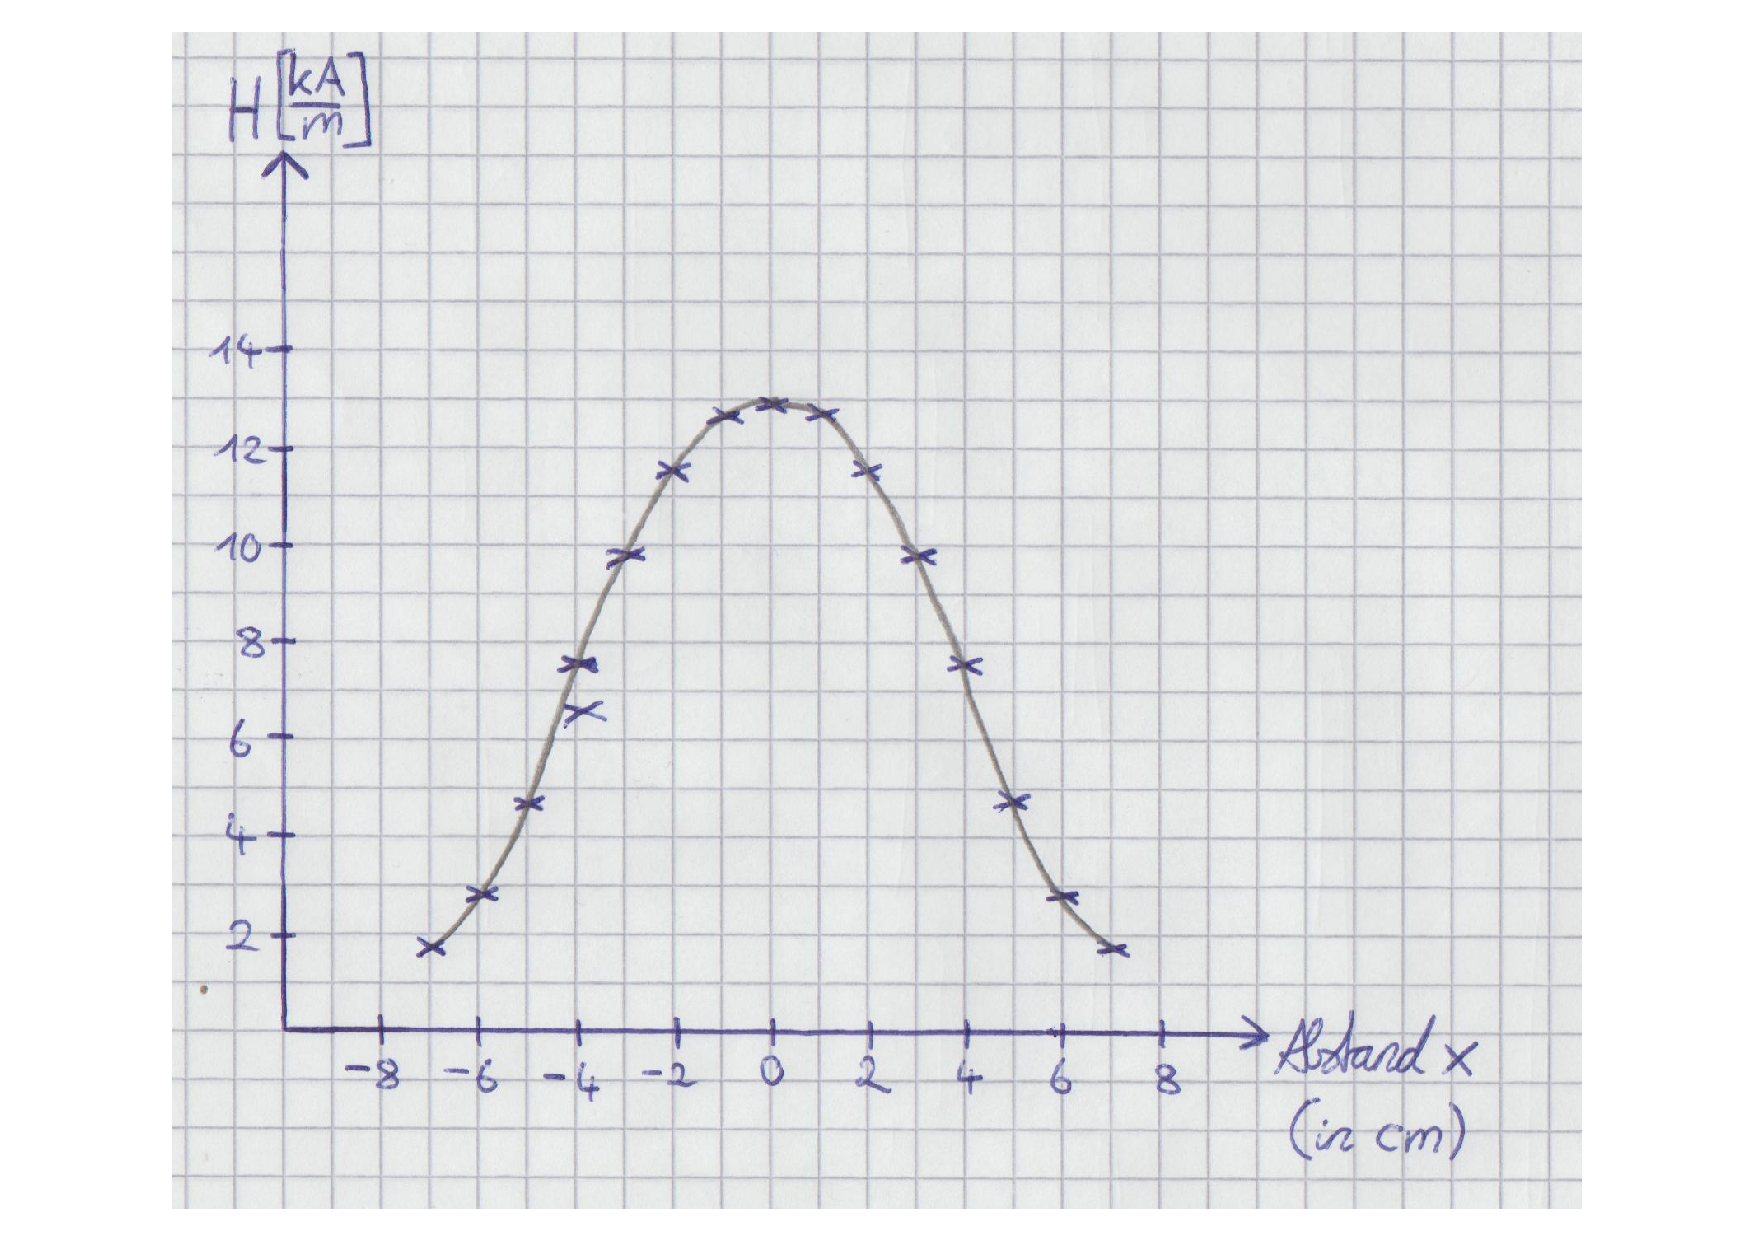
\includegraphics[width=0.9\textwidth]{./Bilder/fma14}
\caption{Skizze Aufgabe 14}
\end{figure}
\FloatBarrier
\subsection{Aufgabe 15}
Betrag des Endmagnetfelds: \\
Das Erdmagnetfeld variiert mit dem Breitengrad, an dem die Messung stattfindet. Sein Betrag beträgt am Äquator ungefähr 30 $\mu$T = 0,3 Gauss und an den Polen ungefähr das Doppelte.
\subsection{Aufgabe 16}
Anwendungen von ferromagnetischen Stoffen in der Praxis: \\
Ferromagnete werden unter anderem als Dauermagnete, Elektromotoren, Transformatoren und auch als magnetische Datenspeicher verwendet. Modernstes Beispiel für Datenspeicherung mithilfe von Ferromagneten ist Fe-RAM, Ferroelectric RAM.

	
\end{document}
